\section{Synchronization Problem}
Another problem for binary 1D CA is the \textit{synchronization problem}.
From some arbitrary initial configuration,
the CA should find its way to a two-step cyclic attractor where all cells share the same state in one timestep,
then all share the other state in the next timestep.
It is thus similar to the majority problem in the way information must be transmitted across the CA in order to coordinate the cells,
but instead of having to "count" cells and landing in a specific point attractor, it finds a cyclic attractor without concern for which of the two states it visits first.

The fitness evaluation function for this experiment is based on the one described in \cite{das1995evolving}, with some modifications.
$K=100$ random initial CA configurations of size $n=49$ are generated from a uniform distribution.
Each candidate solution is first tested on $I=25$ initial configurations.
Each test has a maximum of $2*n$ iterations before being stopped.
If none of the $I$ configurations results in the desired behavior, a fitness of $0.0$ is reported.
If any of the configurations does result in the desired behavior, the candidate is tested on all $K$ configurations.
The fitness reported is then the fraction of configurations that results in the correct behavior.

\subsection{Results}
\begin{table}
\centering
\begin{tabular}{c|c}
Rate & \# \\\hline
0.94 & 1 \\
0.95 & 2 \\
0.96 & 2 \\
0.97 & 65 \\
0.98 & 27 \\
0.99 & 3 \\
1.0 & 0 \\
\end{tabular}
\caption{Distribution of max fitness achieved in 100 independent trials}
\label{tbl:synchronization_training}
\end{table}

Table \ref{tbl:synchronization_training} shows the distribution of the best achieved fitness in the 100 independent trials.
None of the trials achieved 100\% coverage of the configurations, but three trials managed to solve all except one.
95 out of 100 trials achieved 0.97 or greater.
Because of the uniform distribution the initial configurations are sampled from,
it is to be expected that a lot of the configurations are similar in that a behavior that can solve one of them can solve many of them.
It is therefore not surprising to find scores greater than $0.9$ early.
The challenge is to be able to solve all the tricky configurations and get the last few tests right.

The method of fitness evaluation used during evolution does not create an absolute measure of fitness unless the set of tests contains all $2^n$ possible initial configurations.
After the evolution is finished, new test configurations are created to re-assess the performance.
This way the solutions can be tested on different grid sizes as well.
Testing on new configuration of various sizes should give a good indication of how general the solutions found are.

To test the performance of the best of each run,
a sample is selected by picking the top 10 performing individuals from each run.
These 1000 individuals are then categorized by CA behavior (as described in Section \ref{sec:behavior}),
and when duplicates are removed, only 48 distinct behaviors remain.
This set of 48 distinct individuals is designated as "candidates" for best solution, and are subjected to the more extensive testing.

\begin{figure}
\centering
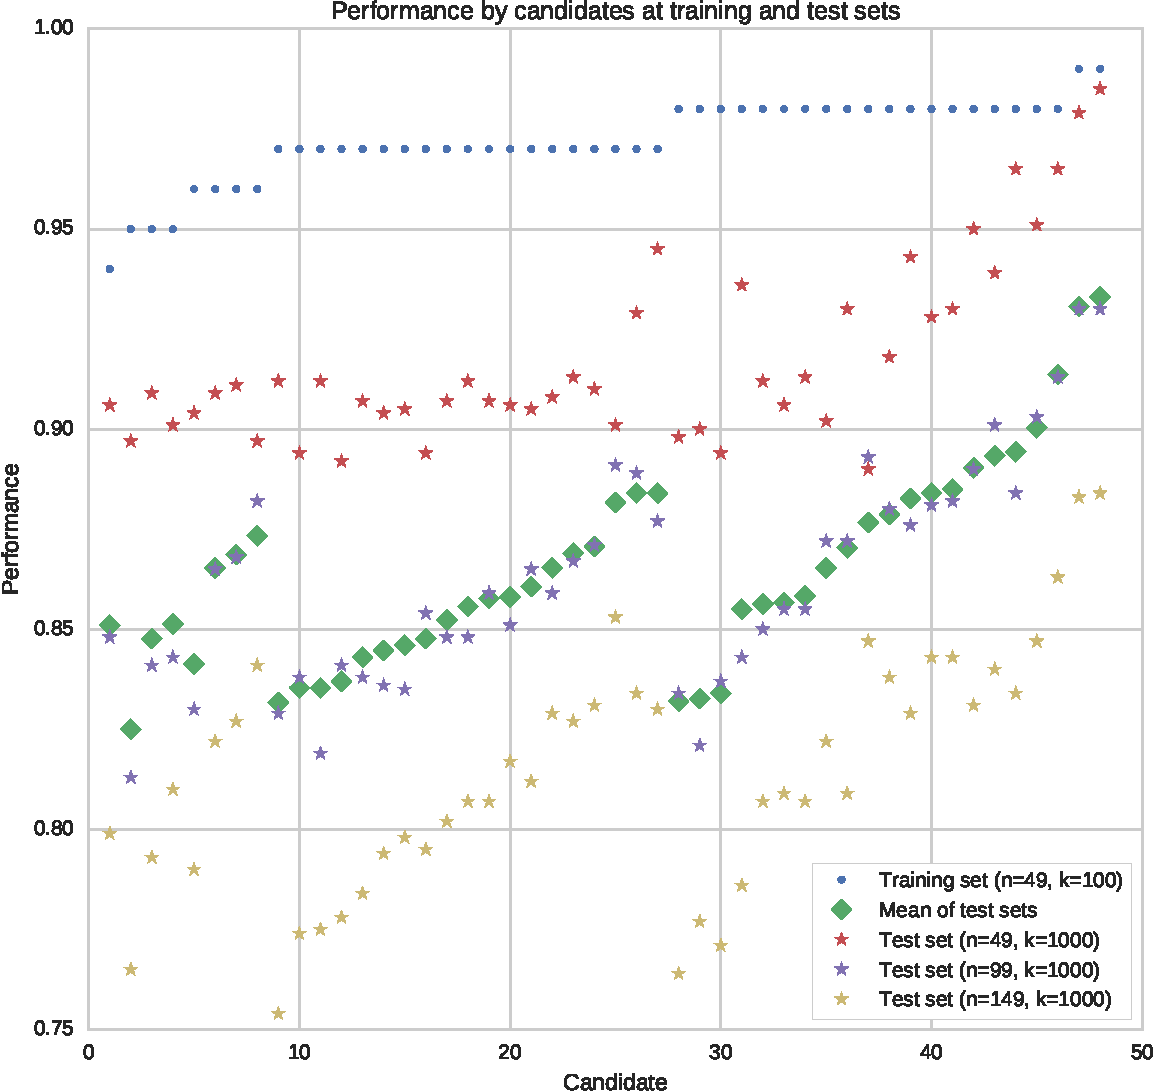
\includegraphics[width=\textwidth, keepaspectratio]{fig/sync_scores}
\caption[
    Performance of the 48 candidate solutions at the training and test sets.
]{
    Performance of the 48 candidate solutions at the training and test sets.
    The candidates have been ordered by training performance first, and average test performance second.
    }
\label{fig:sync_scores}
\end{figure}

Figure \ref{fig:sync_scores} shows the performance of the 48 candidates at the training set and each of the test sets.
It is clear that the candidates that have been trained on $n=49$
There is a correlation between the average score of the test sets and $n$, with the $n=49$ test performing closest to the $n=49$ training performance.
It is also clear that the two candidates that performed the best ($f=0.99$) at the training set, also perform the best at each of the test sets.

